\documentclass[12pt]{article}

\usepackage[utf8]{inputenc}
\usepackage[a4paper,top=2.1cm,bottom=2.1cm,left=2.4cm,right=2.4cm]{geometry}
\usepackage{graphicx}
\usepackage{setspace}
\usepackage{tabularx}
\usepackage{xcolor}
\usepackage{amsmath}
\usepackage{amssymb}
\usepackage[backend=biber,style=numeric]{biblatex}
\usepackage[pdfpagelabels]{hyperref}
\usepackage{mdframed}
\usepackage{subcaption}

\addbibresource{main.bib}

% custom commands
\newcommand{\todo}[1]{{\color{red}#1}}
\newcommand{\comment}[1]{}
% shorthand command aliases
\newcommand{\fancy}{\mathcal}

\begin{document}

\begin{titlepage}
       \Large
       \begin{center}
           
\includegraphics[width=0.4\textwidth]{imgs/logo.png}
       \end{center}
       \renewcommand{\thepage}{Title}
       \thispagestyle{empty}
          \begin{center}
              \vspace*{1cm}
       \linespread{1.25}
              {\doublespacing \Huge\textbf{$\epsilon$-Differential Privacy and Low-Population Histogram Estimation}}
       \linespread{1}
              \vspace*{0.5cm}
              \rule{\linewidth}{1pt}
              \vspace*{1em}
              {\huge Bachelor Thesis \\
              \Large Department of Mathematics and Computer Science, \\
              University of Southern Denmark}
       \end{center}
       \vspace{2cm}
       \Large
       \begin{tabularx}{\textwidth}{lXr}
           Author & & Johan Fagerberg \\
           Supervisor & & Jacopo Mauro \\
       \end{tabularx}
       
       \vfill
       \begin{center}
           \large \today
       \end{center}
       \end{titlepage}


\renewcommand{\abstractname}{Abstract}
\begin{abstract}
\todo{Todo}
\end{abstract}

\begin{center} \bf Keywords \end{center}

\thispagestyle{empty}
\tableofcontents
\newpage

\section{Introduction}

Privacy-preserving data collection has long been an area of interest for many, but never before has it seen as significant focus as it has over the last few decades. With the advent of the Internet, and the global shift towards highly connected lifestyles that comes with it, data can now be gathered from almost every aspect of our lives---and with that comes a need to guarantee subject privacy.

For a long time this has been attempted primarily through techniques that ``anonymizes'' incoming data, attempting to remove any information that may lead to privacy loss. Unfortunately this approach has shown itself to be fallible: without formal guarantees, it relies on the foresight of the data analysts who decide what data to remove, which often leads to de-anonymization when auxiliary data---or simply insufficient anonymization---is present.

\bigskip

In recent years, an alternative approach has emerged in the form of \emph{differential privacy}. By introducing a formal description of "privacy loss", differential privacy not only offers a way to describe and compare differentially private algorithms, but also guarantees that the privacy provided by such algorithms does not falter in the presence of unforeseen auxiliary information or attack approaches.

In this \todo{thesis?} we will be exploring the definition of differential privacy, the guarantees it provides (and which ones it doesn't), and how common statistical problems are solved in differentially private ways. We will put particular focus on what's known as \emph{local differential privacy}. Finally, we will be exploring one particular algorithm for differentially private telemetry collection.

\section{Differential privacy}

\subsection{Motivation}

\begin{description}
    \item[Setting] Interactive vs. non-interactive.

    \item[Privacy] We want to guarantee subject privacy (yet to be defined). Doing so requires defining what "private data" means---historically this has been done on a case-by-case basis, with the privacy guarantees being given against an attacker with some defined abilities and knowledge. This falters under unforeseen circumstances, such as auxiliary information or new capabilities.
    
    \item[Historical] At the time (2006) the prevailing approach was ``anonymizing'' the data through removing "personally identifiable information". What was and wasn't removed was largely decided on a case by case basis. Example: any of the numerous examples of US states releasing ``anonymized'' medical data, only to later be re-identified.
    
    Another approach that had been largely dormant for a few decades, but was gaining steam in the previous few years, was perturbing the data through random noise. This gives subjects privacy through plausible deniability. Example: randomized response.
    
    \item[Differential privacy] It is in this context that diff priv came to be. Following a line of research into noise-based perturbation, differential privacy aims to provide a formal measure for how much noise should be added. As it turns out, the specific approach used offers some interesting guarantees, which we will explore later.
\end{description}

\subsection{Differential privacy \label{sec:promise}} 

\begin{description}
    \item[Differential privacy] Formulated in 2006 by Dwork et al. \cite{dworketal2006}. Gives a formal measure for a specific definition of ``privacy'' in algorithms (any process that takes our dataset and provides an output). Relies on the intuition that an algorithm cannot violate the privacy of someone whose data isn't used in it. If we could guarantee each subject that the output of our algorithm wouldn't change regardless of whether their data was used, then there wouldn't be any risk of privacy breaches from using their data.
    
    We can't actually guarantee that; revealing nothing while providing utility is impossible as proven in \cite{dwork2006_diffpriv}. Rather, we can quantify how close to this ``perfect'' notion we are.
    
    Specifically, for any two databases $D_1$ and $D_2$ differing in only one entry,
    \begin{equation}
        \Pr[\fancy{K}(D_1) \in S] \leq \exp(\epsilon) \cdot \Pr[\fancy{K}(D_2) \in S]
    \end{equation}
    
    \item[Privacy definition] It's worth exploring what this definition of privacy means. The guarantee that ``anything we reveal could (essentially) be revealed without your data'' doesn't mean that we won't reveal anything about our subject. Classic example of car insurance agent: our study may reveal that one of our subjects has a higher risk of being in traffic accidents due to being young, but it \emph{cannot} reveal any information that's specific to the subject---if knowledge of the subject in particular is required, then our subject cannot reveal it.
    
    \item[Meaning of $\epsilon$:] $\epsilon$ is considered the ``privacy budget'' of the algorithm in question (also called ``privacy measure'', ``privacy parameter'', \dots). An algorithm offering differential privacy at a given $\epsilon$ is called an $\epsilon$-differentially private algorithm.
    
    $\epsilon$ is a measure of how much privacy loss is permitted for any one entry, with high values permitting high privacy loss, and low values protecting subject privacy well. As it is used as an exponent, high values of $\epsilon$ quickly get out of hand---a $10$-differentially private algorithm allows for one of the outputs to be 22000 times more likely than the other, while a $2$-differentially private algorithm only allows up to 7 times.
    
    Generally we want low values of $\epsilon$ to protect subject privacy, but this naturally also means more noise, meaning our output will generally be farther from the true answer. As such, the goal is to find a low $\epsilon$ that still permits useful conclusions from the output. The specifics of such a tradeoff depend on the specific output form (\todo{TODO: find papers to reference for e.g. counting queries, histograms, \dots}).
    
    Failing to reach some specific level of $\epsilon$-differential privacy does not necessarily mean that the algorithm is not private. For example, the algorithm may simply be $2\epsilon$-differentially private---something that is essentially identical for low values of $\epsilon$. Even for high values of $\epsilon$, failing to meet the guarantee can mean anything from being essentially differentially private except for one output, to blatant privacy violations (e.g. releasing the dataset directly).
\end{description}

\subsection{Composition theorems}

One of the great bonuses of differential privacy is that we can formally describe how much privacy loss we incur when combining or using differentially private algorithms.

\begin{description}
    \item[Immunity to post-processing] Any algorithm that only uses the output of an $\epsilon$-differentially private algorithm is itself $\epsilon$-differentially private. For the post-processing function $f$ and the set of outputs $T=\{ r | f(r) \in S \}$ we have:
    \begin{align*}
        \Pr[f(\fancy{K}(D_1)) \in S] &= \Pr[\fancy{K}(D_1) \in T] \\
        &\leq \\
        \Pr[f(\fancy{K}(D_2)) \in S] &= \Pr[\fancy{K}(D_2) \in T],
    \end{align*}
    meaning that if $\fancy{K}$ is $\epsilon$-differentially private, then so is $f \circ \fancy{K}$.
    
    This proves it for deterministic functions. Can be extended to randomized functions \todo{(using method I don't understand; they can be decomposed into convex combination of deterministic functions, and a convex combination of diff priv functions are also diff priv?)}
    
    This is crucial because it formalizes an important aspect of our privacy guarantees. With this immunity we know that our guarantees cannot be compromised or harmed after the fact, by anyone who does not have access to our original dataset---unlike e.g. data sanitation techniques that may be de-anonymized later using linkage attacks.
    
    \item[Linear combination] Given both an $\epsilon_1$-differentially private algorithm $f(x)$ and an $\epsilon_2$-differentially private algorithm $g(x)$, their combination $h(x) = (f(x), g(x))$ is $\epsilon_1+\epsilon_2$-differentially private.
    \begin{align*}
        \frac{\Pr[h(x) = (r_1, r_2)]}{\Pr[h(y) = (r_1, r_2)]} &=\frac{ \Pr[f(x)=r_1]\Pr[g(x)=r_2]}{\Pr[f(y)=r_1]\Pr[g(x)=r_2]} \\
        &= \left( \frac{\Pr[f(x)=r_1]}{\Pr[f(y)=r_1]} \right) \left( \frac{\Pr[g(x)=r_2]}{\Pr[g(y)=r_2]} \right) \\
        &\leq \exp(\epsilon_1) \exp(\epsilon_2) = \exp(\epsilon_1 + \epsilon_2)
    \end{align*}
    
    This can be extended to the combination of any number of algorithms.
\end{description}

\subsection{Achieving differential privacy}

\begin{description}
    \item[Laplace] For numeric functions (i.e. $f : \mathbb{N}^n \to \mathbb{R}^k$) we can make them differentially private by adding suitable noise to their output. The Laplace mechanism is one way of doing this.
    
    An important measure is the $\ell_1$-sensitivity of the function, defined as
    \begin{equation}
        \Delta f = \underset{\begin{subarray}{c}
            x,y \in \mathbb{N}^{n} \\
            ||x-y||_1 = 1
        \end{subarray}}{\max} || f(x)-f(y) ||_1,
    \end{equation}
    i.e. the biggest difference any one entry can have on the output. Intuitively we could mask the contribution of any one entry by adding noise of this size.
    
    Another important definition for the Laplace mechanism is the Laplace distribution, whose density function is defined as
    \begin{equation}
        \text{Lap}(b,x) = \frac{1}{2b} \exp \left( -\frac{|x|}{b} \right).
    \end{equation}
    
    Using this we can define create our $\epsilon$-differentially private function as
    \begin{equation*}
        f'(x) = f(x) + (Y_1, \dots, Y_k)
    \end{equation*}
    where $Y_i$ are independent random variables drawn from $Lap(\Delta f/\epsilon)$.
    
    \item[Exponential] The exponential mechanism is used for cases where the task is to choose the ``best'' response out of multiple choices. It does not add noise to the output, but rather 
\end{description}

\subsection{Variants of differential privacy}

\begin{description}
    \item[$(\epsilon, \delta)$-differential privacy] The guarantee of $\epsilon$-differential privacy is strong. In some cases it may be practical to weaken our guarantee a bit, e.g. to allow rare events to impact our output beyond what would be allowed normally.
    
    A variant of differential privacy, called $(\epsilon, \delta)$-differential privacy \cite{dwork2006_delta_diffpriv}, alters the definition slightly, such that for any two neighboring datasets $D_1$ and $D_2$,
    \begin{equation}
        \Pr[\fancy{K}(D_1) \in S] \leq \exp(\epsilon) \cdot \Pr[\fancy{K}(D_2) \in S] + \delta.
    \end{equation}
    
    This definition allows algorithms that may not live up to the stronger guarantee of $\epsilon$-differential privacy (or which have large $\epsilon$ measures under that definition) to provide this weaker guarantee instead.
    
    This guarantee differs in some significant ways from the one provided by $\epsilon$-differential privacy. It allows the differential privacy guarantee to ``fail'' sometimes, giving outputs that---in the worst case---leak the presence (or absence) of the entry in question. For example, it allows the algorithm to have an output that \emph{never} happens, unless a particular entry is present---in which case it has a probability of at most $\delta$. If such an output is given, an attacker will know for certain that the entry is present.
    
    This is naturally undesirable. As such, low $\delta$ values are desired for $(\epsilon, \delta)$-differentially private algorithms, as this limits the likelihood of our privacy guarantee ``failing''. It is worth noting that the desirable range for $\delta$ depends on the population size. The likelihood of of a ``failure'' is at most $\delta$ for each entry in the dataset. As this guarantee is given independently for each entry, the expected probability of ``failure'' for any of our $n$ entries is $\delta \cdot n$---since we do not want this to happen, our $\delta$ must generally be smaller if we work on larger datasets.
    
    \item[Local differential privacy] Also known as ``randomized response''. Indicates that the perturbation of data is done client-side, such that nothing can be learnt about a subjects true answer even with full knowledge of the individuals reported answer.
\end{description}

\section{Experiments with low-population telemetry collection}

\subsection{Introduction}

A 2017 paper building on a local differentially private algorithm for repeatedly collecting metrics from subjects. Historically an issue has been that privacy guarantees quickly degrade over repeated collections, e.g. when collecting telemetry over time.

\subsection{Introduction/Historical context}

\subsection{Low population experiments}

\begin{description}
    \item[Experiment setup] We wish to explore the effect of low population size on the utility of the mean and histogram estimation mechanisms described in \cite{microsoft_telemetry}. The paper tests the estimation errors of population sizes varying from $0.3\times10^6$ to $3\times10^6$, but does not test the errors for lower population sizes than this; this leaves many applications---such as telemetry collection by smaller companies than Microsoft---with little information on the applicability of the mechanisms.
    
    We test both estimation mechanisms on synthetic datasets sampled from constant, uniform and (truncated) normal distributions, similar to those used in the empirical evaluation in the paper.
    
    \item[Mean estimation]
    
    \item[Histogram estimation]
    We aim to measure the \emph{histogram error} of the estimated histograms, defined as $\max_{v\in[k]} |\hat{h}(v)-h(v)|$ where $\hat{h}(v)$ is the estimated frequency of the bucket $v$, and $h(v)$ is the true frequency. This is the error measure used in the paper. In addition to this we also measure the Wasserstein distance between the true and the estimated histograms (with any negative values in the estimated histogram truncated to 0). The histogram error is used to measure the maximum error of any one bucket in the histogram. The Wasserstein distance is used to measure the distance of the entire histogram to the true values.
    
    In order for our results to be comparable to those of the original paper, we use similar parameters beyond the population size: we use $k=32$ evenly sized buckets on the range $[0,24]$, permanent memoization for repeated collection, but no output perturbation. We vary population size in the range $[10^3, 3\times10^5]$ and $\epsilon$ in the range $[0.1, 10]$. In order to minimize the impact of the random nature of the mechanisms, we calculate the metrics by averaging over 10 separate estimations.
    
    The results can be seen in figure \ref{fig:histogram_errors}. As expected, low population sizes give significantly worse estimation errors: at $n=10^4$ and $\epsilon=1, d=1$ the average estimation error for our normal dataset is $0.3$, compared to just $0.045$ when $n=3\times10^5$. In other words, the bucket with the largest misestimation was off by $30\%$ at $n=10^4$. At $n=3\times10^5$ no bucket was misestimated by more than $4.5\%$.
    
    Depending on the use case of the estimated histograms, it may be difficult to know the impact of the histogram error on the utility of the histogram. For the purpose of achieving a more intuitive understanding of the estimation error, a visual representation of the histogram estimation for our normal dataset can be seen in figure \ref{fig:histogram_matrix}. The Wasserstein distance is a formal measure similar to this intuitive understanding, and reflects many of the same attributes: at low enough $\epsilon$ values the ``utility'' of the histograms does not improve throughout the tested population sizes. Similarly, at high $\epsilon$ values the measure improves only slightly. In between these two the ``utility'' improves from poor to acceptable as we approach the larger population sizes. We expect the measure for all the tested $\epsilon$ values to approach 0 as population size increases further.
    
    \begin{figure}
        \centering
        \makebox[\textwidth][c]{
            \subcaptionbox{Normal distribution}
                {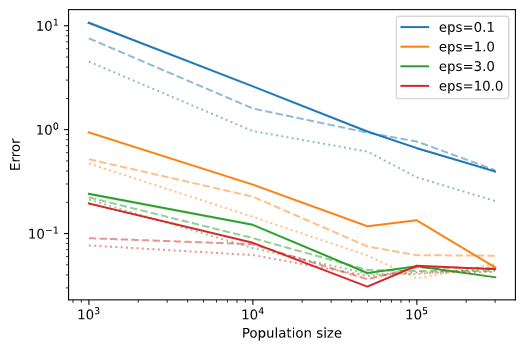
\includegraphics[width=0.6\textwidth]{imgs/histogram_err_normal.png}
                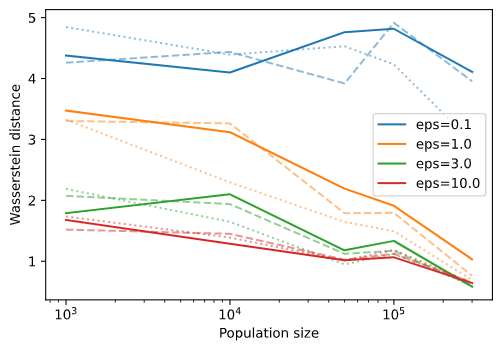
\includegraphics[width=0.6\textwidth]{imgs/histogram_wassersteins_normal.png}}
        }
        \makebox[\textwidth][c]{
            \subcaptionbox{Uniform distribution}
                {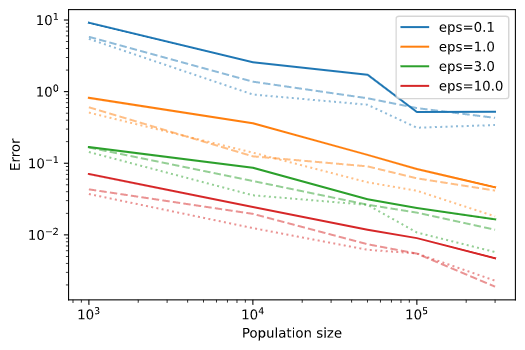
\includegraphics[width=0.6\textwidth]{imgs/histogram_err_uniform.png}
                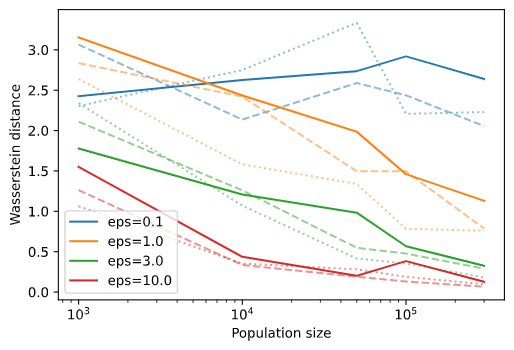
\includegraphics[width=0.6\textwidth]{imgs/histogram_wassersteins_uniform.png}}
        }
        \makebox[\textwidth][c]{
            \subcaptionbox{Constant distribution}
                {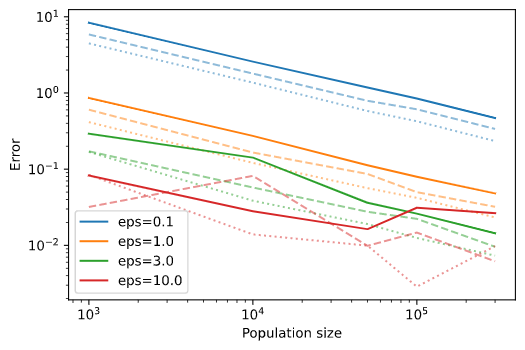
\includegraphics[width=0.6\textwidth]{imgs/histogram_err_constant.png}
                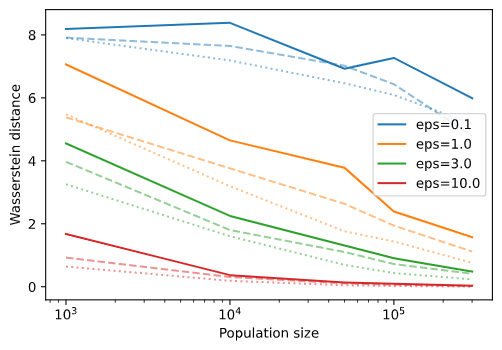
\includegraphics[width=0.6\textwidth]{imgs/histogram_wassersteins_constant.png}}
        }
        \caption{Estimation errors for the histogram estimation mechanism at various $\epsilon$ and population sizes. Solid, dashed and dotted lines are $d=1,2,4$ respectively.}
        \label{fig:histogram_errors}
    \end{figure}
    
    
    
    \begin{figure}
        \centering
        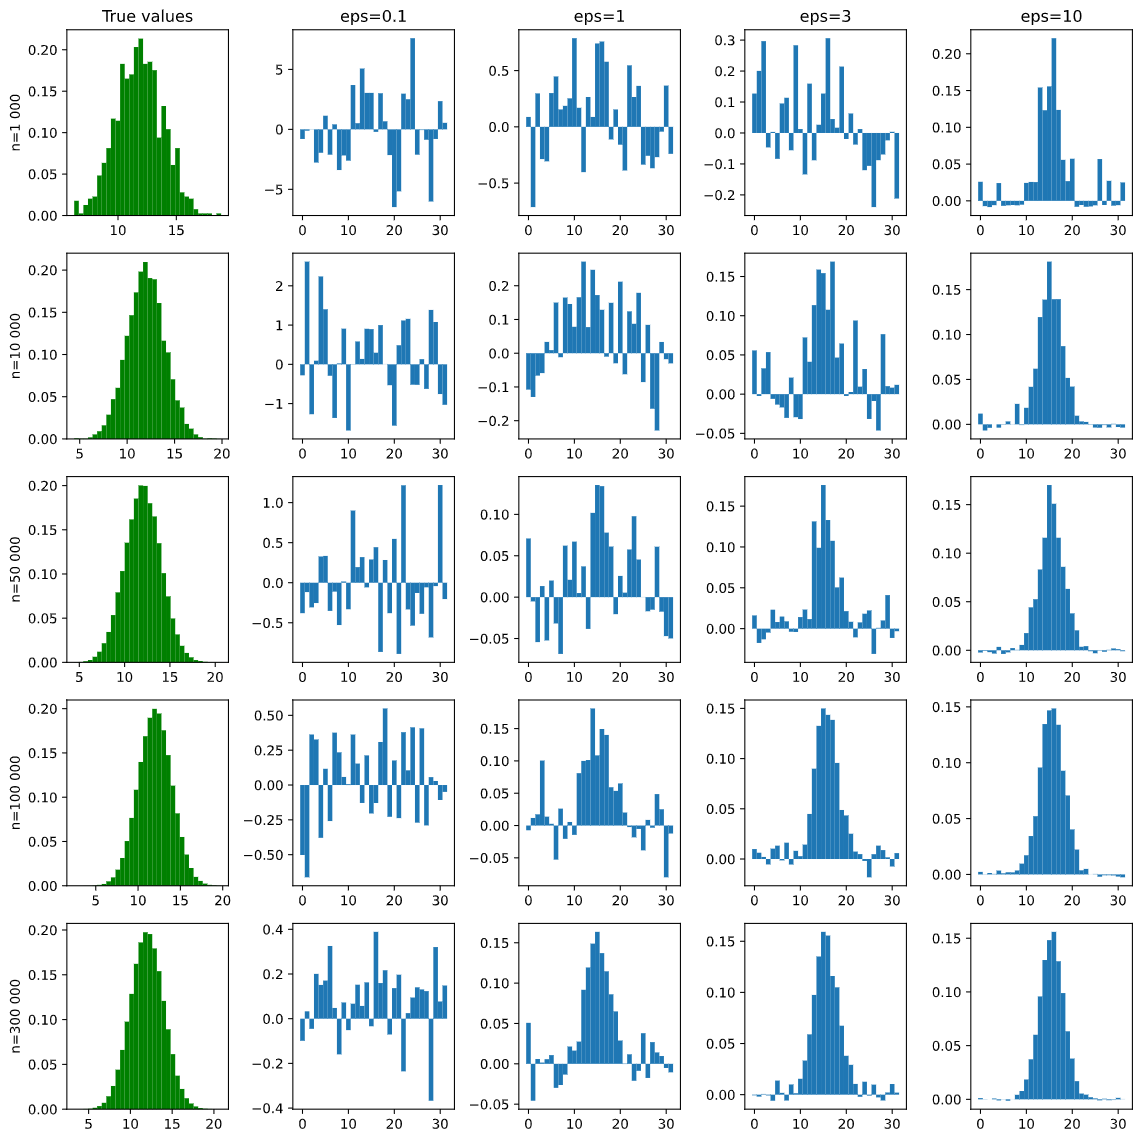
\includegraphics[width=\textwidth]{imgs/histogram_matrix.png}
        \caption{Examples of estimated histograms for various $\epsilon$ and population sizes with $d=1$.}
        \label{fig:histogram_matrix}
    \end{figure}
\end{description}

\subsubsection{Results}

\section{Conclusions}

Summary of results

Discussion of what they mean

Future work

% appendix if needed

\end{document}
